\section{Web Map Tile Service}
Web Map Tile Service merupakan peta ubin yang dikembangkan pertama kali oleh Open Geospatial Constortium (OGC). 
Terdapat potensi di dalam Web Map Tile Services yaitu gambar peta ubin dapat di cache pada lokasi antara klien dan server, 
mengurangi latensi yang terkait dengan proses pembuatan gambar. Lapisan ubin biasanya di pasang di sisi server, menyajikan 
ubin gambar peta secara bersamaan ke beberapa pengguna. Selain itu, banyak pemetaan klien, seperti Google Earth atau Nasa 
World Wind, telah menyematkan cache, yang juga dapat mengurangi kemacetan jaringan dan penundaan jaringan. \cite{Garc{\'\i}a2002Webmap}


\subsection{Skema Ubin}
Peta sudah lama dikenal hanya seperti yang tercetak di atas kertas. Peta kartografi tercetak tersebut merupakan representasi 
statis yang terbatas pada skala visualisasi tetap dengan Tingkat Detil tertentu (LOD). Namun, dengan perkembangan peta digital, 
pengguna dapat memperbesar atau mengurangi area yang divisualisasikan dengan melakukan pembesaran operasi, dan LOD diharapkan 
dapat diperbarui sesuai dengan itu. 

Adaptasi konten peta sangat bergantung pada skala: Peta skala kecil berisi informasi yang kurang rinci daripada peta skala besar 
di wilayah yang sama. Proses mengurangi jumlah data dan menyesuaikan informasi dengan skala yang diberikan disebut generalisasi 
kartografi, dan biasanya dilakukan oleh server peta web.

Untuk menawarkan layanan peta web ubin, server peta web membuat peta melintasi serangkaian skala tetap melalui generalisasi yang 
progresif. Gambar peta yang dirender kemudian dibagi menjadi ubin, menggambarkan piramida ubin seperti yang digambarkan pada
gambar \ref{TilePyramid.JPG} 

\begin{figure}[ht]

\centerline{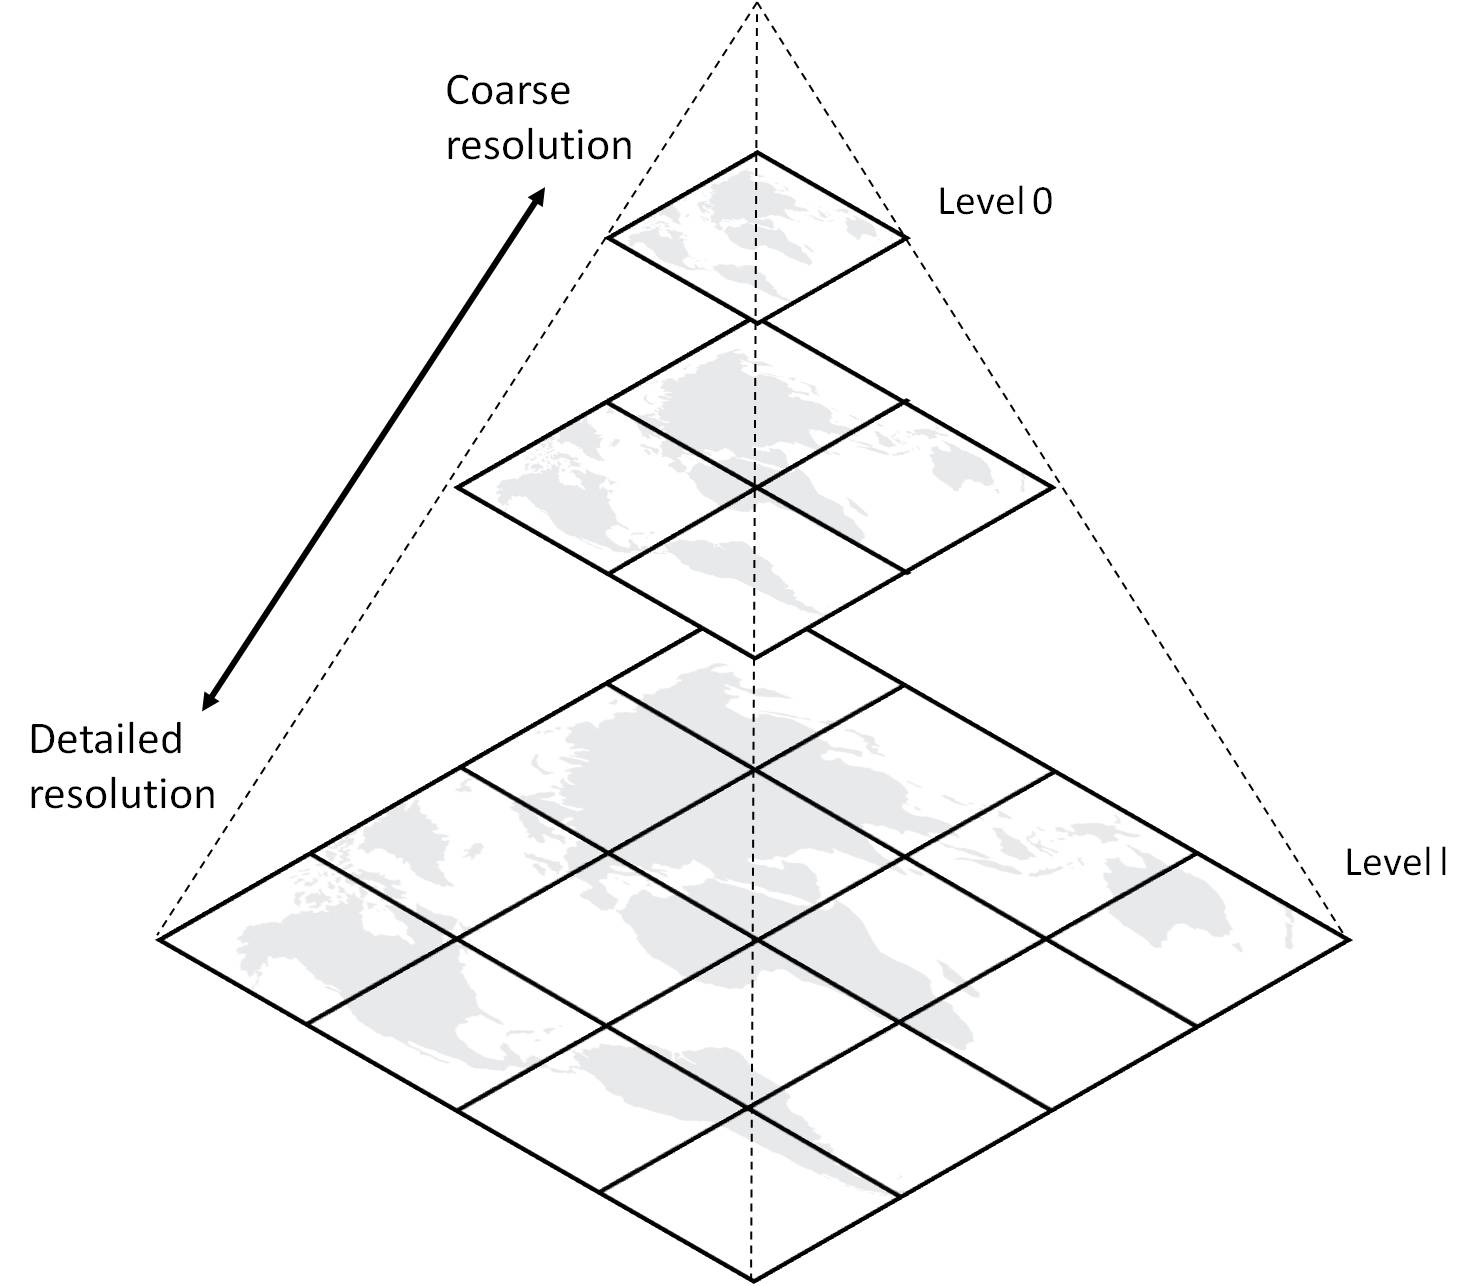
\includegraphics[width=1\textwidth]{figures/TilePyramid.JPG}}

\caption{Representasi piramida ubin}

\label{TilePyramid}

\end{figure}

gambar \ref{TilePyramid.JPG} merupakan contoh skema ubin dari Microsoft Bing Maps dimana tingkat pertama memungkinkan mewakili 
seluruh dunia dalam 4 ubin (2x2) dari  256x256 piksel. Tingkat berikutnya mewakili seluruh dunia dalam 16 ubin (4x4) dari 256x256 
piksel dan seterusnya sampai tingkat 4. \cite{Garc{\'\i}a2002Webmap}

